\documentclass[12pt, letterpaper, titlepage]{article}
\usepackage[utf8]{inputenc}
\usepackage{geometry}
\usepackage{color,graphicx,overpic} 
\usepackage{fancyhdr}
\usepackage{amsmath,amsthm,amsfonts,amssymb}
\usepackage{mathtools}
\usepackage{hyperref}
\usepackage{multicol}
\usepackage{array}
\usepackage{float}
\usepackage{blindtext}
\usepackage{longtable}
\usepackage{scrextend}
\usepackage[font=small,labelfont=bf]{caption}
\usepackage[framemethod=tikz]{mdframed}
\usepackage{calc}
\usepackage{titlesec}
\usepackage{listings}
\usepackage[normalem]{ulem}
\usepackage{tabularx}
\usepackage{mathrsfs}
\usepackage{bookmark}
\usepackage{setspace}
\usepackage{booktabs}
\usepackage{tikz}
\usepackage{pgfplots}
\pgfplotsset{width=8cm,compat=1.15}\usepgfplotslibrary{patchplots}
\mathtoolsset{showonlyrefs}  
\allowdisplaybreaks

\definecolor{mycolor}{rgb}{0, 0, 0}

\geometry{top=2.54cm, left=2.54cm, right=2.54cm, bottom=2.54cm}
\setlength{\headheight}{20pt}
\setlength{\parskip}{0.3cm}
\setlength{\parindent}{1cm}

\pagestyle{fancy}
\fancyhf{}
\rhead{Lora Ma - 1570935}
\lhead{\textit{ECE 322 Lab 2}}
\rfoot{Page \thepage}

\begin{document} 
\singlespacing

\section{Introduction}
The purpose of this lab was to become familiar with several black-box testing techniques. The techniques introduced in this lab were Extreme Point Combination (EPC), and weak n x 1 testing. We will be testing two Java programs -- Drone and RemoteCar. In EPC testing, we complete a single domain analysis for a given subdomain in order to identify the domain limits for each dimension. Then, we can choose test cases for each domain -- max, min, slightly under min, and slightly over max. Another additional test case is added within the valid subdomain. Together, this is $4^n + 1$ cases, where $n$ is number of input variables. In weak nx1 strategy, we try to find linear boundaries of the problem using domain analysis. In domain analysis, $n$ points are selected on each linear boundary, where $n$ is the amount of input variables. One additional point is also chosen outside of each boundary. If the boundary is open, then all points on the boundary receive exterior processing. In this case, choose an additional point within the boundary. If the boundary is closed, then all points on the boundary receive interior processing. In this case, choose an additional point outside the boundary. This strategy produces $b(n+1)+1$ test cases, where $b$ is the number of linear boundaries, and $n$ is the number of input variables.

\section{Part One - Drone program}
\subsection{Q1}
For task one, the Drone application was tested using EPC and weak nx1 strategy. Drone is a new GPS-enabled automated pilot system being testing for unmanned reconnaissance aircraft. The system controls the unmanned aircraft from takeoff to landing. The unmanned aircraft has enough fuel to reach a max distance $k$ before needing to return back to base. The aircraft can have a travel a max of 3 waypoints $x_1, x_2, x_3$. In this experiment, $k$ is 100. Therefore, $x_1 + x_2 + x_3 \leq k$ where $x_1, x_2, x_3$ must be $\geq 0$. The program should output "Success" if it is successful and "Failure" if it is not. 

\subsection{Q2}
Looking at all the failed test cases, we can see that whenever $x_2$ is negative, the output is "Success" when it should be "Failure". For the EPC testing strategy, we were able to see 2 types of failures, when the output is incorrectly "Success" or "Failure". For the weak nx1 strategy, we were only able to see when "Success!" is incorrectly outputted.

\subsection{Q3}

\begin{figure}[H]
  \centering
  \begin{tikzpicture}
  
  \begin{axis} [
      view = {60}{15},
      xmin = 0,
      xmax = 100,
      ymin = 0,
      ymax = 100,
      zmin = 0,
      zmax = 100,
      xlabel = $x_1$,
      ylabel = $x_2$,
      zlabel = $x_3$,
      xtick = {0, 50, 100},
      ytick = {0, 50, 100},
      ztick = {0, 50, 100},
      grid,
      colormap/bluered
  ]
  
  \addplot3 [
      opacity = 0.5,
      table/row sep = \\,
      patch,
      patch type = polygon,
      % fill = teal,
      faceted color = red,
      vertex count = 3,
      patch table with point meta = {
          0 1 2 0 \\
          0 1 3 1 \\
          0 2 3 2 \\
          1 2 3 3 \\
      },
  ] table {
      x y z \\
      0 0 0 \\
      0 0 100 \\
      0 100 0 \\
      100 0 0 \\
  };
  
  \end{axis}
  \end{tikzpicture}
  \caption{Subdomain of all valid inputs for drone program}
  \end{figure}
  \subsection{Q4}
  The EPC approach was able to find 2 different types of failures whereas the weak nx1 approach was only able to find 1 type of failure. The two types of failures seem to have stemmed from the same issue (when $x_2 < 0$), so although the weak nx1 approach was unable to find both types, it was able to still find the primary issue causing both of the problems. It seems like weak nx1 testing is more efficient in finding problems since the weak nx1 approach was able to find it with 17 test cases compared to the 65 test cases that the EPC approach required.

\newpage
\subsection{Q5}
EPC Testing - Drone

\includegraphics[scale=0.82]{image1.png}
\newpage
Weak nx1 Testing - Drone

\includegraphics[scale=0.88]{image2.png}

\section{Part 2 - Remote Car Program}
\subsection{Q1}
For task 2, we tested a remote-controlled car piloting system using EPC and weak nx1 testing. The car may not be any more than a distance r from the origin. The program takes Cartesian inputs in the form of (x, y) which specify where the car should move. The point must fall on the circle with radius 1, centered around the origin. If it is, the program will output "Ok"; otherwise, it will output "Out of range".

\subsection{Q2}
We approximated the circle using four linear equations: 
\begin{equation}
  y = \begin{cases}
      x + 1 & -1 \leq x \leq 0 \\
      -(1+x) & -1 \leq x \leq 0 \\
      x - 1 & 0 \leq x \leq 1 \\
      1-x & 0 \leq x \leq 1 \\
  \end{cases}
\end{equation}
\subsection{Q3}
For the EPC testing we had $4^2 + 1 = 17$ tests. No tests failed during EPC testing and seemed more effective in testing the circle subdomain than weak nx1 testing.

The weak nx1 domain approximation seemed not very effective. It had 4 errors out of the 13 tests. It worked best if test inputs are chose quite far away from the boundaries, since it's possible for there to be a false negative if a input is chosen too close to the boundary. This is possible when test values are chosen just outside the approximated boundary. If we increased the number of lines, the number of test cases would also increase, and the accuracy would increase. Weak nx1 testing requires $b(n+1)+1$ tests, where $b$ is the number of segments and $n$ is the amount of input variables. If we used 12 segments, we would have $12(2+1)+1 = 37$ test cases.

For this situation, EPC testing is more accurate than weak nx1 testing. Weak nx1 had 4 test case failures out of 13 due to the linear approximation of the subdomain. No actual errors were found in the application. EPC testing had no test failures despite having a similar number of tests as weak nx1 testing. With more segments, weak nx1 testing will be more accurate.

\subsection{Q4}
EPC Testing - Remote Car

\includegraphics[scale=1]{image3.png}

\newpage
Weak nx1 Testing - Remote Car

\includegraphics[scale=1]{image4.png}

\section{Conclusion}
In this lab, we were introduced to two black box testing techniques -- Extreme Point Combination (EPC), and weak nx1 testing. We tested two Java programs -- Drone and Remote Car.

In part 1, we tested the Drone program. When applying EPC testing, we found 9 failed test cases. When applying weak nx1 testing, we were only able to find 1 failed test case. These errors stemmed from the same one problem and both testing methods were able to find it. The problem we found was when $x_2 < 0$. In part 2 we tested the Remote Car program. When applying EPC testing we found no failed test cases; however when applying weak nx1 testing, we found 4 failed test cases. These test case failures were because of the linear approximation we used when applying weak nx1 testing. It was difficult to know if the program wasn't working properly or the testing was not working as intended. 

One testing strategy is not better than the other. It is better to choose the testing strategy appropriate for the program being tested for the best results. The weak nx1 strategy seems to excel when the problem is already linear so no linear approximation is needed. With the linear approximation, weak nx1 testing is a lot less reliable. EPC works really well in situations that weak nx1 strategy is not so good at. Although there are many more test cases, EPC testing seems more accurate. It didn't produce any false positive cases and more failures in the program were found than in weak nx1 testing. 
\end{document}